\chapter{StrepHit}
\label{cha:strephit}
La terza parte del progetto consiste nell'implementazione di uno script in Python (versione 2.7) che, dato in input un dataset di QuickStatements, deve restituire in output il dataset
arricchito con nuovi riferimenti.

Ogni riga del dataset di input presenta una proprietà \href{https://www.wikidata.org/wiki/Property:P854}{reference URL} (P854) con l'URL di riferimento della risorsa, lo 
script deve eseguire una query SPARQL per trovare l'item nel knowledge base che corrisponde al dominio della URL e la proprietà di tale item che definisce lo schema della URL in questione.

\subsection{Esempio di funzionamento}
Per esempio dato il seguente quickstatement in input:
\begin{lstlisting}[style=QuickstatementsStyle, caption=Riga del dump]
    Q193660	P106	Q207628	S854	"http://www.nndb.com/people/031/000097737/"
\end{lstlisting}

Notiamo una prima relazione semantica 
\href{https://www.wikidata.org/wiki/Q193660}{\code{Q193660}} (Ramon Llull) \href{https://www.wikidata.org/wiki/Property:P106}{\code{P106}} (occupation) 
\href{https://www.wikidata.org/wiki/Q207628}{\code{Q207628}} (musical composition) 
che ci dice semplicemente che \lq\lq \textit{Ramon Llull lavora come compositore musicale}\rq\rq .

Segue la proprietà che interessa maggiormente \code{S854 "http://www.nndb.com/people/031/000097737/"} che indica la provenienza dell'informazione. 

Lo script procede estrapolando il dominio dalla reference url (\code{www.nndb.com}) e con una query sparql trova l'item di riferimento a quel dominio in Wikidata, sempre che esista.

In questo caso l'item di riferimento è \href{https://www.wikidata.org/wiki/Q1373513}{Q1373513} che fra le varie proprietà presenta anche una Wikidata property (\code{P1687}) chiamata  
\lq\lq \textit{NNDB people ID}\rq\rq\ (\code{P1263}).

Se ora analizziamo la proprietà \lq\lq \textit{NNDB people ID}\rq\rq\ (\code{P1263}) notiamo che presenta una proprietà formatter URL (\code{P1630}) il cui valore è \code{http://www.nndb.com/people/$\$1/$}. 
Il valore finale \code{$\$1$} nella formatter URL è un placeholder che sta ad indicare la parte della URL che corrisponde al valore della proprietà prescelta. 

Lo script andrà quindi ad estrapolare dalla URL di partenza il valore \code{031/000097737} che corrisponde al valore della proprietà \code{P1263} e andrà ad arricchire il dump 
con questa informazione aggiuntiva.

\begin{lstlisting}[style=QuickstatementsStyle, caption=Risultato dello script]
    Q193660	P106	Q207628	S854	"http://www.nndb.com/people/031/000097737/"	S248	Q1373513	S1263	"031/000097737"	S813	2018-06-04T02:19:10Z/14
\end{lstlisting}

I riferimenti aggiuntivi sono: 
\href{https://www.wikidata.org/wiki/Property:P248}{\code{S248}} (stated in)
\href{https://www.wikidata.org/wiki/Q1373513}{\code{Q1373513}} (NNDB)
\href{https://www.wikidata.org/wiki/Property:P1263}{\code{S1263}} (NNDB people ID)
\code{"031/000097737"} (il valore estrapolato, people ID)
\href{https://www.wikidata.org/wiki/Property:P813}{\code{S813}} (retrieved)
\code{2018-06-04T02:19:10Z/14} (timestamp).

\section{SPARQL Query}
Per risolvere ogni dominio e ogni formatter URL sconosciuta si usa una sola query; si è cercato di limitare il più possibile il numero di query effettuate 
(dato che alcune query possono impiegare svariati secondi ad essere eseguite), 
salvando in memoria e su disco i risultati di quelle già lanciate in precedenza per minimizzare il tempo di computazione dello script.

\begin{lstlisting}[style=SPARQLStyle, caption=SPARQL query per cercare item e proprietà relativi al dominio \code{"www.nndb.com"}]
    select Distinct ?subjects ?wikidataProperty ?formatterUrlLabel ?sitelinkLabel
    where {
        {
            BIND("www.nndb.com" AS ?domain).
            SERVICE wikibase:label { bd:serviceParam wikibase:language "[AUTO_LANGUAGE],en". }
            ?subjects wdt:P856 ?sitelink ;
                      wdt:P1687 ?wikidataProperty.
            ?wikidataProperty wdt:P1630 ?formatterUrl
            FILTER (REGEX(str(?formatterUrl), ?domain) || REGEX(str(?sitelink), ?domain)).
        }
        union
        {
            BIND("www.nndb.com" AS ?domain).
            SERVICE wikibase:label { bd:serviceParam wikibase:language "[AUTO_LANGUAGE],en". }
            ?subjects wdt:P856 ?sitelink ;
            FILTER REGEX(str(?sitelink), ?domain).
        }
    }
\end{lstlisting}

Va premesso che esistono molti modi di ottenere lo stesso risultato, con costrutti molto meno verbosi, tuttavia questa è l'unica query che attualmente non manda in timeout l'endpoint.

Il superamento del timeout è sicuramente dovuto al fatto che internamente si usano delle regular expressions che appesantiscono molto l'esecuzione della query, soprattutto su 
grandi knowledge base come quello di Wikidata. 

In SPARQL usare una ricerca per stringa è certamente una forzatura perchè solitamente si conoscono già a priori item e propery che interessano tuttavia in questo caso è 
stato necessario adottare la ricerca per regular expression dato che lo script deve proprio affrontare il problema inverso.

La query è il risultato dell'unione di due sub-query; la prima sub-query cerca tutte le proprietà che posseggono una proprietà formatter URL (P1630) il cui valore ha come dominio il 
dominio del quickstatement che lo script sta analizzando (in questo caso "www.nndb.com"); in oltre controlla che tale priprietà sia legata ad un item il cui official website (P856) 
sia coerente con il dominio in questione. 

La seconda sub-query invece cerca solo tutti gli item il cui official website (P856) abbia lo stesso dominio di quello del quickstatement che lo script sta analizzando. 
Questa query è necessaria perchè non sempre esiste una proprietà la cui formatter URL matcha correttamente con il link che si sta analizzando; può succedere che esista solo l'item 
relativo al database in questione ma non la proprietà specifica e in pochi casi non esiste nemmeno tale item. In alcuni casi invece può succedere che l'item relativo al database 
esista ma abbia un dominio completamente differente da quello della proprietà la cui formatter URL presenta un match con la URL in analisi. 

La difficoltà principale nella realizzazione dello script è stata proprio quella di gestire una moltitudine di casi particolari derivanti dal fatto che il dataset era molto grande
(più di 500.000 quickstatements) con una svariati domini differenti e qualche URL completamente sbagliata o deprecata. 

\begin{center}
    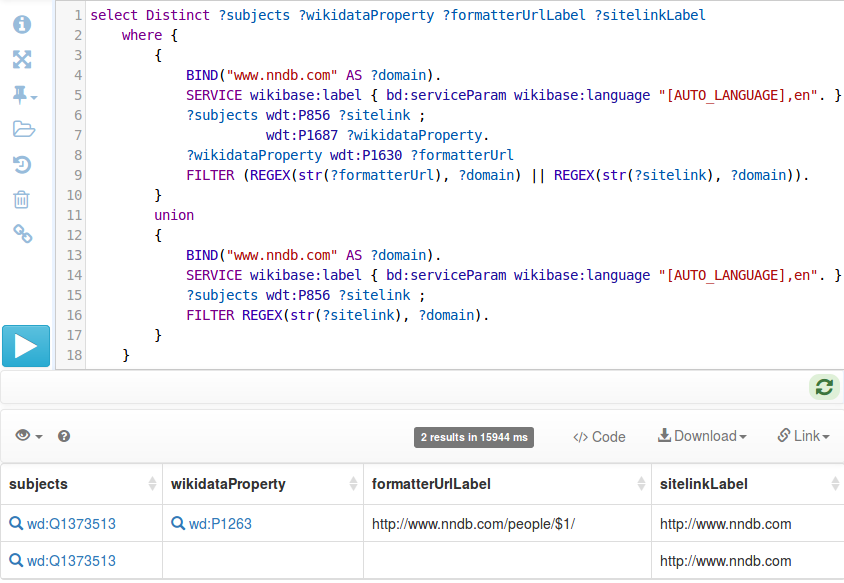
\includegraphics[width=\linewidth]{Sources/Img/c04_01.png}
    \captionof{figure}{Risultato della query per il dominio \code{"www.nndb.com"}}
\end{center}

\section{Lo script}

\subsection{Struttura del progetto}
Il progetto presenta una cartella assets contenente tutti i file di input e output, i json di configurazione e i log degli errori; nella cartella business sono contenuti i servizi,
i metodi di utilità e le query. 

La cartella domain contiene i modelli e le localizations (nel file localizations.py sono definite anche una serie di costanti da settare a seconda 
delle esigenze per configurare lo script). 

In tests abbiamo tutte le classi di test basate sulla libreria unittest, come per il Client $C\#$ anche in questo caso è stato configurato Travis per far eseguire i test 
automaticamente ad ogni pull-request. 

Infine nella root del progetto abbiamo l'entry point dello script (main.py) e l'entry point dei test (test.py), i requirement per il package manager 
e il file di configurazione strephit.py nel caso si voglia lanciare lo script in un virtualenv tramite la libreria click.

\subsection{Algoritmo}
Istanziando l'oggetto QuickStatementsService vengono caricati automaticamente in memoria i mappings presenti nella cartella assets; 
i mappings sono dei file json di salvataggio in cui lo script salva i risultati delle le chiamate, all'end-point SPARQL, già effettuate.

\begin{lstlisting}[style=jsonStyle, caption=Some Code]
    "www.nndb.com": [
        {
            "db_id": "Q1373513", 
            "db_property": "S1263", 
            "to_upper_case": false, 
            "url_pattern": "http://www.nndb.com/people/$1/"
        }
    ], 
\end{lstlisting}

Il metodo \code{add\u db\u references\u async()} cicla su ogni riga del dataset e per ogniuna di esse chiama un handler (\code{add\u db\u references\u async\u handler()}), passandogli un oggetto 
QuickStatement contenente tutte le informazioni della riga, che procede con l'analisi della URL e la generazione dei riferimenti mancanti.

A questo punto, in modo sincrono o asincrono, a seconda del settaggio delle costanti in localizations.py (\code{IS\u ASYNC \u MODE = True/False}), 
viene chiamato il metodo \code{generate\u db\u reference()} che provvede a controllare che nei mappings ci sia già una entry con formatter URL compatibile 
con la URL del quickstatement e a generare i riferimenti mancanti.

Se nei mappings non esiste nessuna entry compatibile con la URL allora viene chiamato il metdo \code{new\u mapping()} che provvede a chiamare l'end-point SPARQL 
e a selezionare il risultato migliore per aggiungerlo ai mappings. 

Se la costante \code{MAP\u ALL\u RESPONSES} viene settata a \code{True}, ogni risposta del endpoint SPARQL viene salvata interamente nei mappings, questo previene qualsiasi altra chiamata all'endpoint 
per un determinato dominio ma accresce la dimensione dei mappings a dismisura e rende di conseguenza la ricerca più lenta.
 
\subsection{Refresh delle URL}
Nel dataset analizzato alcuni domini erano deprecati tant'è che tentando di accedervi da un browser si veniva reindirizzati ad altri domini oppure era avvenuto il passaggio da http ad https.

Per non perdere questi riferimenti si è deciso di implementare anche una funzionalità che data una lista di domini va a refreshare tutte le URL aventi tali domini e ad eliminare le 
righe contenenti URL inesistenti.

A fine procedura vengono salvati i log con la lista di url modificate e con la lista di righe eliminate dal dataset.

